\documentclass[a4paper,12pt,openright,twoside]{report}
\usepackage[utf8]{inputenc}
\usepackage[italian]{babel}
\usepackage{pdflscape}
\usepackage{afterpage}
\usepackage{esvect}
\usepackage{amsthm}
\usepackage{graphicx}
\usepackage{indentfirst}
\usepackage{stmaryrd}

\theoremstyle{definition}
\newtheorem{es}{Esempio}[section]

\begin{document}

\chapter{Introduzione}
TODO

\chapter{Titolo da decidere}
In questo capitolo viene introdotta la \emph{Sentiment analisys}, di cosa si occupa e
il motivo per cui si sta diffondendo in maniera cosi rapida.
Successivamente vengono descritti, in maniera generale, i vari strumenti utilizzati
in questa tesi in particolare \emph{RNNLM}, \emph{word2vec} e \emph{Liblinear}.

\section{Sentiment Analisys}
Con il termine \emph{Sentiment analysis} e \emph{opinion minig}, si intende uno studio 
che analizza le opinioni, i sentimenti, le valutazione e le
emozioni del linguaggio scritto utilizzato dalle persone.
E' una delle aree di ricerca più attive nel campo dell'analisi del linguaggio
naturale ma allo stesso modo si estende anche nell'ambito del \emph{data mining} e
\emph{text mining} ossia quella branca di ricerca riguardante l'estrazione di un sapere o di una conoscenza a partire da grandi quantità di dati.
Di fatto, questo tipo di ricerca, nato nell'ambito dell'informatica si è diffusa
ampiamente in rami diversi come ad esempio: la scienza sociale,
l'economia, le aziende e multinazionali nonchè l'intera società che ci circonda.

Questa enorme diffusione della \emph{sentiment analysis} conicide con la 
crescita dei cosidetti \emph{social media}: siti di commercio e recensioni di prodotti,
discussioni su forum, blog, micro-blog, Twitter e i vari \emph{social network}.
Per la prima volta nella storia  è stato possibile disporre di una
enorme quantità dati digitalizzati da manipolare, analizzare e studiare in maniera
estremamente approfondita, al fine di estrapolare ed ottenere un'analisi
ampiamente sfaccetta e particolareggiata.

I sistemi di \emph{sentiment analysis} sono utilizzati in quasi tutti
le attività del cosidetto dominio sociale poiché le opinioni e i pareri sono il centro
di quasi tutte le attivita umane e anche la chiave che influenza il nostro 
comportamento.
Quello in cui crediamo, la percezione della realtà, le scelte che facciamo,
sono condizionate dai giudizi degli altri
riguardo noi stessi e dall'ambiente che ci circonda. 
Per questo motivo, quando abbiamo bisogno
di prendere una decisione, spesso cerchiamo il parere e il consenso altrui.
Infine, possiamo notare, che questo comportamento è vero non solo 
per i singoli individui ma allo stesso modo lo vediamo
applicato ad organizzazioni, aziende e grandi multinazionali.
Da tutti questi aspetti è facile dedurre 
come questo tipo di analisi possa avere una grande influenza nel mondo che 
ci circonda sia dal punto di vista economico che sociale.

La linguistica e l'analisi del linguaggio naturale (NLP) hanno una lunga
storia, mentre per quel che riguarda la \emph{sentiment analysis} le prime ricerca
è sono state svolte a partire dell'anno 2000; da quel momento questo campo è diventato un'area
di ricerca estremamente attiva. 
Le ragioni che hanno portato \emph{sentiment analysis}
crescita cosi immediata e su cosi larga scala sono: per prima cosa le applicazioni
di cui dispone questo tipo di ricerca, possono essere utilizzate in un ampio raggio di 
situazioni e domini differenti. Ciò ha generato un aumento di interessi
con un relativo stanziamento di finanziamenti verso questo tipo di ricerca che ha portato ad una prolificazione di 
applicazioni commerciali e ad una costante ricerca alla soluzione di problemi
che fino ad ora non erano stati ancora studiati.
Infine la crescita esponenziale dell'ultimo decennio è dovuta all'enorme 
quantità di dati fornita dal web dove, per la prima volta nella storia, è stato possibile
raccogliore milioni di dati riguardati opinioni, idee e pareri di persone o intere 
popolazioni.
Senza questa mole di dati è facile pensare come la maggior parte delle ricerche non
sarebbero state possibili.

\subsection{Applicazioni della Sentiment Analysis}
Partendo dal presupposto che le opinioni e i pareri sono la base di tutte le attivita sociali perché sono la chiave
che influenza il nostro comportamento.
Nel mondo reale, aziende e multinazionali sono costantemente alla 
ricerca di giudizi e pareri, riguardo i loro prodotti, da parte dei consumatori.
Allo stesso modo il consumatore vuole avere informazioni riguardo agli articoli da
acquistare, pareri riguardo un determinato film o un nuovo album musicale etc.
In passato quando un'azienda necessitava di un parere del consumatore effettuava sondaggi
d'opinione o gruppi di discussione; ottenere questo tipo di dati è stato per lungo
tempo un grande business per aziende di marketing, le pubbliche relazioni e le compagnie pubblicitarie.

Al giorno d'oggi chiunque voglia comprare un prodotto, non è più limitato a dover chiedere
ad amici o famigliari perché può trovare centinaia di recensioni o discussioni online.
Allo stesso modo per un'azienda non è più necessario condurre sondaggi, o analisi di mercato
visto l'enorme diffusione dei dati disponibili.
Tuttavia la ricerca, l'estrazione e l'annotazione di questi dati è un compito di una complessita non indifferente.
Basti pensare alla quantità di informazioni scritte in un post di un blog o in un forum,
perfino una persona ha difficoltà nel riassumere ed estrarre le informazioni utili da questo
tipo di testo. Ecco perché diventa cosi importante uno studio finalizzato e strutturato in un 
determinato ambito.

\section{Recurrent neural Networks}
Gli esseri umani non iniziano a pensare da zero ogni secondo, per esempio il lettore, leggendo questa tesi,
associa il significato di ogni parola basandosi si quelle lette in precedenza. Questo concetto viene anche 
definito come la persistenza della memoria.

Le reti neurali tradizionali non funzionano in questo modo ed ignorano gli eventi passati. Per esempio 
volendo classificare gli eventi che succedono in ogni punto di fuilm non e' chiaro come una rete neurale
possa utilizzare gli eventi passati per classificare quelli correnti.

Per cercare di risolvere questo problema sono state create le \emph{reccurent neural networks (RNN)},
a differenza delle reti neurali tradizionali le \emph{RNN} hanno dei cicli interni che permettono
all'informazione di persistere 

\begin{figure}[h]
	\centering
	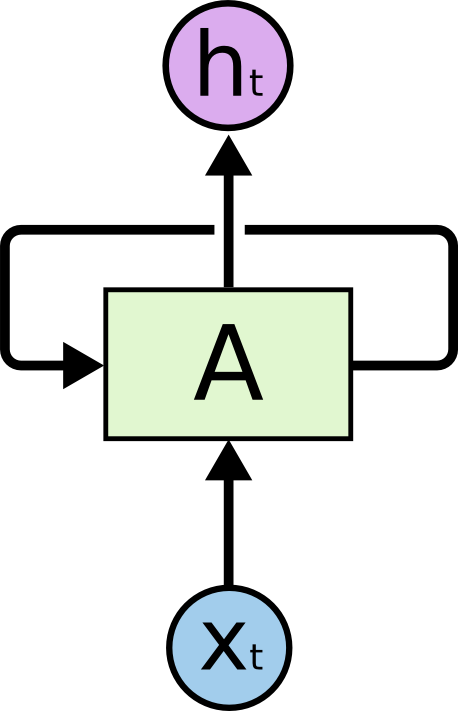
\includegraphics[scale=0.5]{Immagini/rnn1.png}
	\caption{Ciclo interno di una RNN}
	\label{fig:rnn1}
\end{figure}

Nella figura \ref{fig:rnn1}, e' rappresentata una rete neurale $A$ riceve in input un valore $x_t$ e genera in output un valore $h_t$.
Un ciclo permette all'informazione di passare da ogni step della rete al successivo. In altro parole possiamo immaginare
una \emph{RNN} come molteplici copie della stessa rete, ognuna che passa un messaggio alla rete successiva.

\begin{figure}[h]
	\centering
	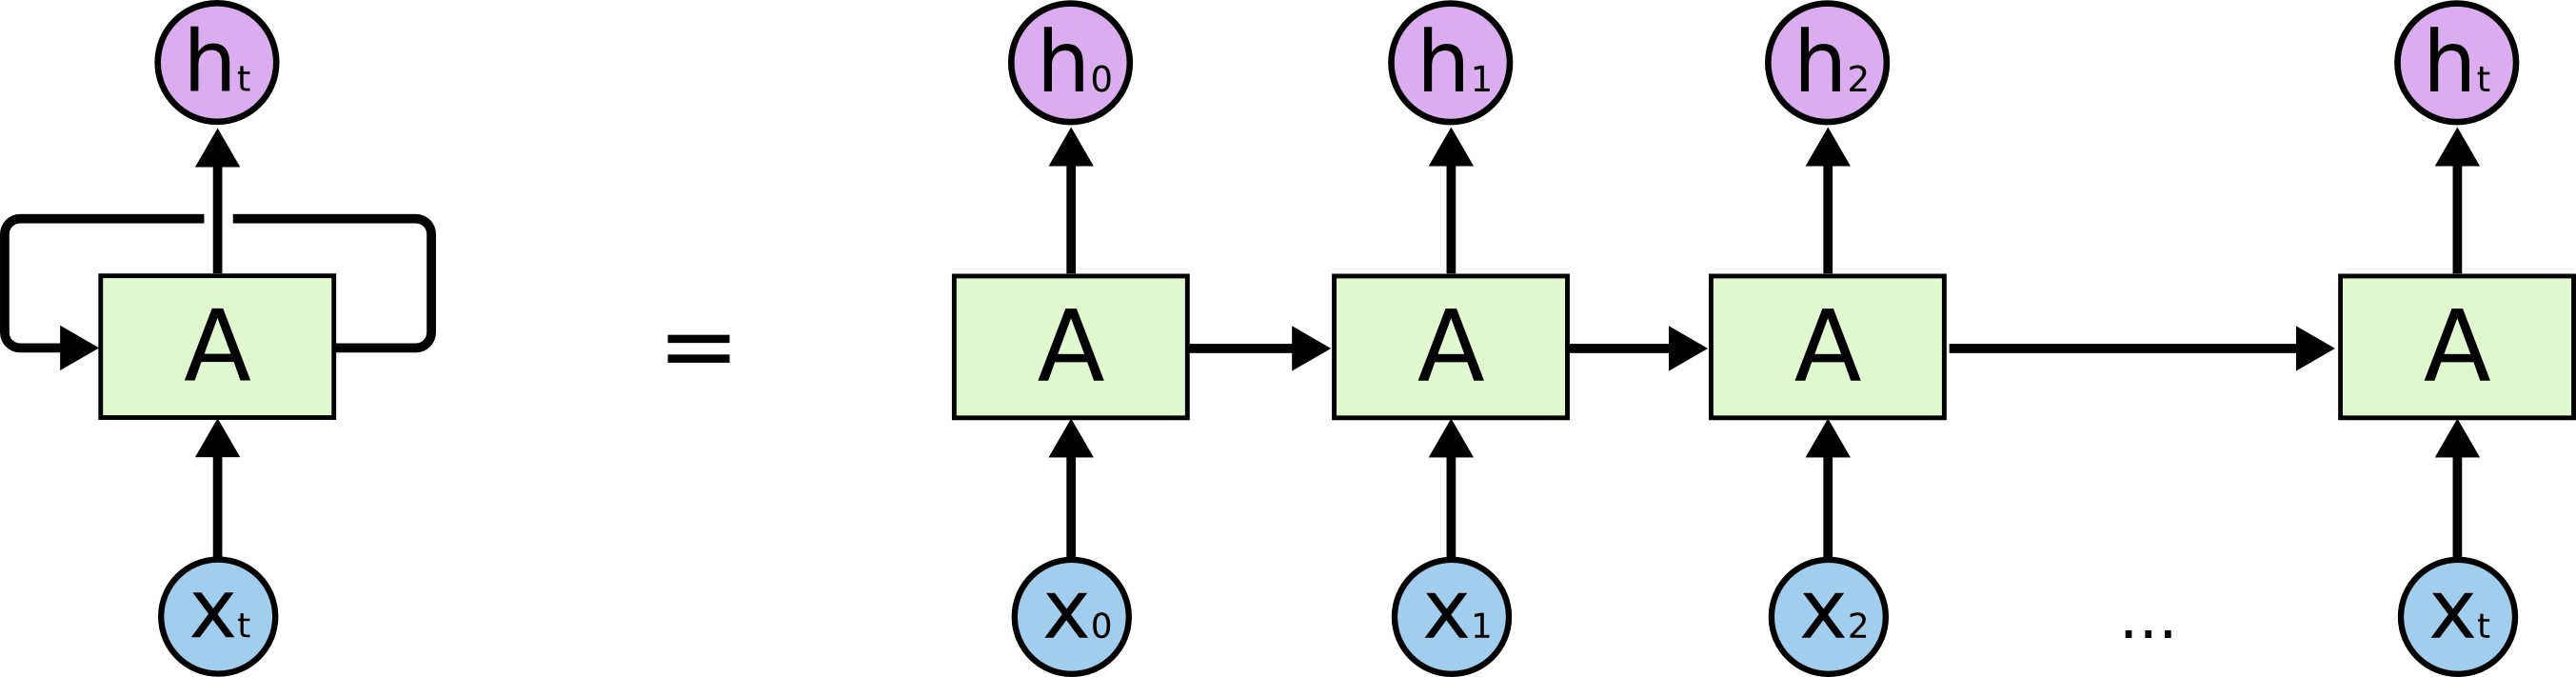
\includegraphics[scale=0.3]{Immagini/rnn2.png}
	\caption{Esempio di RNN rimuovendo il ciclo}
	\label{fig:rnn2}
\end{figure}

\subsection{RNNLM}
La rete neurale utilzzata per l'analisi dei dati in questa tesi è il toolkit RNNLM. 
L'architettura utilizzata nel toolkit è mostrata in \ref{fig:rnnlm} viene solitamente chiamata rete di Elman o semplicemente RNN. Il layer di input usa una rappresentazione $1-a-N$ delle 
parole precedenti $w(t)$ concatenate con il precedente stato dell'hidden layer $s(t - 1)$.
\begin{figure}[h]
  \centering
      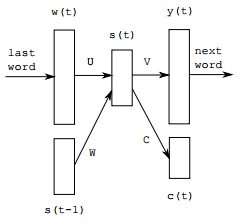
\includegraphics[width=0.5\textwidth]{Immagini/rnnlm_rete.png}
      \caption{Esempio di rete neurale ricorsiva}
\label{fig:rnnlm}
\end{figure}

I neuroni dell'\emph{hidden layer} $s(t)$ usano una sigmoid activation function (todo).
L'output layer $y(t)$ ha le stesse dimensioni di $w(t)$, dopo che alla rete è stato fatto training,
rappresenta la probabilità della distribuzione della parola successiva data la parola precendete 
e lo stato dell'hidden layer nel precedente istante di tempo.
Un class layer $c(t)$ può essere usato per ridurre la complessità del modello ma con un piccola
diminuzione della precisione.
Il training è viene svolto utilizzando un stochastic gradient descent algorithm, e la matrice $W$
che rappresenta il recurrent weights viene calcolata utilizzando la backpropagation throught time algorithm (BPTT).
Specificatamente, su RNNLM, viene utilizzato un truncate BPTT, la rete viene processata solo per uno specifico
numero di time steps.
\subsection{Fase di training}
I dati in input attesi sono sotto forma di un semplice file ASCII, con spazi tra le parole e il carattere di
fine linea al termine di ogni frase.
Una volta specificato il corpus di test, il vocabolario viene costruito automaticamente e viene salvato come parte
del file di modello della RNN.
Nel caso si voglia limitare il vocabolario il file di input deve essere processato esternamente sostituendo
tutte le parole da eliminare con un token speciale (per esempio \textbf{<unk>}.
Una volta che viene generato il vocabolario inizia la parte di training. Oltre al corpus è atteso anche un
file di validazioni dati per controllare il numero di training \emph{epochs} e  il learning rate.
E' possibile fare training di modelli senza utilizzare un file di validazione utilizzando l'opzione \textbf{-one-iter}
\subsection{Fase di test}
Una volta che è stato fatto training sul modello può essere valutato su i dati di test, la perplexity e la 
probabilità $\log_{10}$ viene mostrata come output.
E' possibile effettuare una interpolazione lineare delle probabilità delle parole dato il modello. L'input atteso
da RNNLM è un file contenente una lista di frasi su cui effettuare lo scoring, ognuna anteposta con un identificatore
numerico univoco.
\section{Word2Vec}
Storicamente i sistemi di \emph{natural language processing} trattano le parole come simboli atomici e discreti,
per esempio la parola ``gatto'' può essere rappresentata da \textbf{Id123} e ``cane'' come \textbf{Id453}.
Questa codifica è arbitraria e non fornisce alcuna informazione al sistema riguardo la relazione
che puo' esistere tra due differenti simboli.
Questo significa che il nostro sistema non può utilizzare praticamente nulla di quello che ha imparato
riguardo il ``gatto'' quando sta processando i dati riguradanti il ``cane'' (per esempio il fatto che siano
entrambi animali, che abbiano quattro zampe, etc.).
Inoltre rappresentare le parole sotto forma di identificatoi univoci porta ad avere una base dati sparsa
con la conseguente necessita' di dover ottenere un maggior numero di dati per riuscire a creare un modello
statistico rappresentativo, proprio questa base dati sparsa e' il principale problema che la 
rappresentazione tramite vettori risolve.

\subsection{Vectors space model}
I Vectors space models (VSM) sono rappresentazioni \emph{embedding} di parole in uno spazio vettoriale 
continuo, ovvero dove le parole
semanticamente simili sono mappate in punti vicini, questo metodo si basa sulla distributional hypotesis, 
cioè sul fatto che parole che appaiono in 
un determinato contesto condividono lo stesso significato semantico.

La rappresentazione di parole in uno spazio vettoriale può aumentare le porformance
di un task di analisi del linguaggio naturale e una delle prime
applicazioni in questo campo è datata al 1986 con il lavoro di Rumelharth, Hinton and Williams. Successivamente
questa idea è stata ampiamente utilizzata e ha trovato applicazione in modelli di ricognizione del parlato,
di traduzione automatica, nonchè di numerosi altri tasks quali etc.

Recementemente, Mikolov et al. hanno introdotto il modello skip-gram 
un metodo efficente per ottenere
rappresentazioni vettoriali di parole provenienti da un grande numero di dati testuali non strutturati.

\begin{figure}[h]
	\centering
	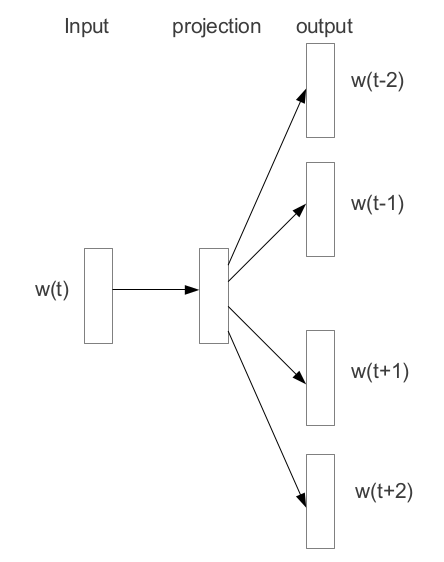
\includegraphics{Immagini/skipgram.png}
	\caption{modello Skipgram. L'obbiettivo e' ottenere vettori di parole capaci di prevedere
	parole simili}
	\label{fig:skipgram}
\end{figure}

Al contrario della maggioranza delle reti neurali utilizzate per la creazioni di vettori di parole, 
il training utilizzando un modello Skip-gram non utilizza moltiplicazioni tra matrici dense,
in questo modo il training diventa estremamente efficiente: una singola macchina può calcolare vettori
partendo da un testo contenente più di 100 miliardi di parole in meno di un giorno.

\subsection{Modello Skip-gram}
Nel modello Skip-gram l'obiettivo di training è quello di creare una vettore di parole che
può essere utilizzate per prevedere parole attorno ad una frase o ad un documento. Più formalmente,
data una seguenza di parole $w_1,w_2,w_3,\dot{},w_T$ definito training l'obbiettivo del modello è quella di aumentare la
probabilità logaritmica:
\begin{equation}
	\frac{1}{T} \sum_{t=1}^{T} \sum_{-c\leq j\leq c,j\neq0} \log p(w_t+j|w_t)
	\label{eq:prob log}
\end{equation}
Dove $c$ è la dimensione del contesto di training (che può essere una funzione basata sulla parola centrale $w_t$).
Utilizzare un $c$ più grande porta ad avere una precisione maggiore, in questo modo, però, si aumenta anche il 
tempo di training. La formulazione standard del modello Skip-gram definisce $p(w_t+j|w_t)$ usando la funzione
softmax:
\begin{equation}
	p(w_O|w_I) = \frac{\exp(v_{w_O} v_{w_I}}{\sum_{w=1}^{W}\exp(v_w v_{w_I}}
	\label{eq:softmax}
\end{equation}

dove $v_w$ and $v'_w$ sono la rappresentazione vettoriale di ``input'' e ``output'' di $w$ e $W$ è il numero
di parole nel vocabolario.
Questa formualzione, però, non e' difficilmente utilizzabile in sistemi reali
perché il costo per il calcolo di $\nabla\log p(w_O|w_I)$
è proporzionale a $W$, che è spesso è molto grande: $(10^5-10^7 termini)$.

\subsection{Hierarchical Softmax}
Una approssimazione del softmax che è computalmente più efficente è il softmax gerarchico. Questo algoritmo
è stato introdotto nell'analisi del linguaggio naturale da Morin e Bengio; il motivo principale
che porta un aumento di prestazioni
è quello di non dover valutare tutti $W$ nodi di output della rete neurale per ottenere una distribuzione
di probabilità ma solo un numero $\log_2(W)$ di nodi.

Il softmax gerarchico utilizza una rappresentazione ad albero binario per il \emph{layer} di output dove, come foglie,
troviamo le $W$ parole e, in ogni nodo, sono rappresentate le probabilità dei nodi figli.
Questo definisce un random walk per assegniare la probabilità alle parole.

Piu' precisamente ogni parola $w$ puo' essere raggiunta da un determinato percorso partendo dalla radice
dell'albero. Definiamo $n(w,j)$ come il $j$-esimo nodo nel percorso che parte dalla radice fino a $w$ e $L(w)$ come
la lunghezza di questo percorso in modo che $n(w,1) = radice$ e $n(w,L(w)) = w$.
In aggiunta, per ogni nodo interno $n$, definiamo $ch(n)$ come un arbitratio nodo figlio di $n$ e $[x]$ ha il valore $1$ se $x$ e' vero e $-1$ altrimenti.
Quindi il softmax gerarchico definisce $p(w_O|w_I)$ come segue:
\begin{equation}
	p(w|w_I) = \prod_{j=1}^{L(w)-1}\sigma([n(w,j+1)=ch(n(w,j))]\dot v_{n(w,j)} )
	\label{eq:hierarchicalSoftmax}
\end{equation}

dove $\sigma(x) = 1/(1+exp(-x))$. Puo' essere dimostrato che $\sum_{w=1}^W p(w|w_I) = 1$. Questo implica
che il costo per calcolare $\log p(w_O|w_I)$ e $log p(w_O|w_I)$ e' proporzionale a $L(w_O)$ che in media
e' piu' piccolo di $\log W$.
Inoltre, al contrario della formulazione stardand del softmax dove troviamo due rappresentazioni differenti 
$v_w e v_w$ per ogni parola $w$, il softmax gerarchico possiede una sola rappresentazione $v_n$ per ogni nodo $n$
dell'albero binario.

Il tipo di albero utilizzato ha una influenza notevole sulle prestazioni dell'algoritmo, nello specifico
in word2vec è stato utilizzato un albero binario di Huffmann, in questo modo 
abbiamo codici di dimensioni più piccole per le parole usate con maggior frequenza risultando in un training più rapido.
Inoltre è stato osservato che rappgruppare le parole utilizzando la loro frequenza funziona molto
bene come tecnica per aumentare la velocità di calcolo.

\section{Classificatori lineari}
La risoluzione di problemi di classificazione su una mole molto grande di dati è uno dei problemi principali
incontrati in applicazioni quali la classificazione di testi.

Un classificatore lineare, nel campo dell'apprendimento automatico, è diventato una delle tecnologie più
promettenti e più utilizzate; l'obiettivo della 
classificazione statistica è quella di usare le caratteristiche degli oggetti (\emph{Features}) per identificare
a quale classe (o gruppo) appartengono. 
Una classificazione lineare raggiunge questo scopo facendo una decisione sulla classificazione basata sul valore di una combinazione lineare di caratteristiche. 
Le caratteristiche di un oggetto sono anche conosciute come \emph{features} e nel calcolatore sono rappresentati solitamente come un vettore chiamato vettore delle caratteristiche.

Questi classificatori funzionano molto bene per probelmi pratici quali la classificazione di 
documenti e più in generale in problemi che utilizzano un numero molto elevato di \emph{features}

Se definiamo un vettore di \emph{features} con l'identificatore $x^\rightarrow$ allora il punteggio di output
è definito come segue:
\begin{equation}
	y=f(w^\rightarrow \cdot x^\rightarrow = f (\sum_j w_jx_j)
	\label{output score}
\end{equation}

dove $w^\rightarrow$ è un vettore reale pesato (\emph{weight vector}) e $f$ è una 
funzione che converte il prodotto scalare di due vettori nell'input desiderato.
Il \emph{weight vector} viene generato partendo da un inseme di esempi utilizzati come training. Solitamente
la funzione $f$ è una semplice funzione
che effettua il mapping di tutti i valori sopra una certa soglia nella prima classe e gli altri valori nella
seconda classe. Una versione più complessa di $f$ potrebbe fornire una probabilità con cui un particolare
oggetto appartiene ad una certa classe.

L'utilizzo dei classificatori lineari è spesso utilizzata in situazioni dove la velocità di classificazione
è rilevante, specialmente quando $x^\rightarrow$ è sparso.
\begin{figure}[h]
	\centering
	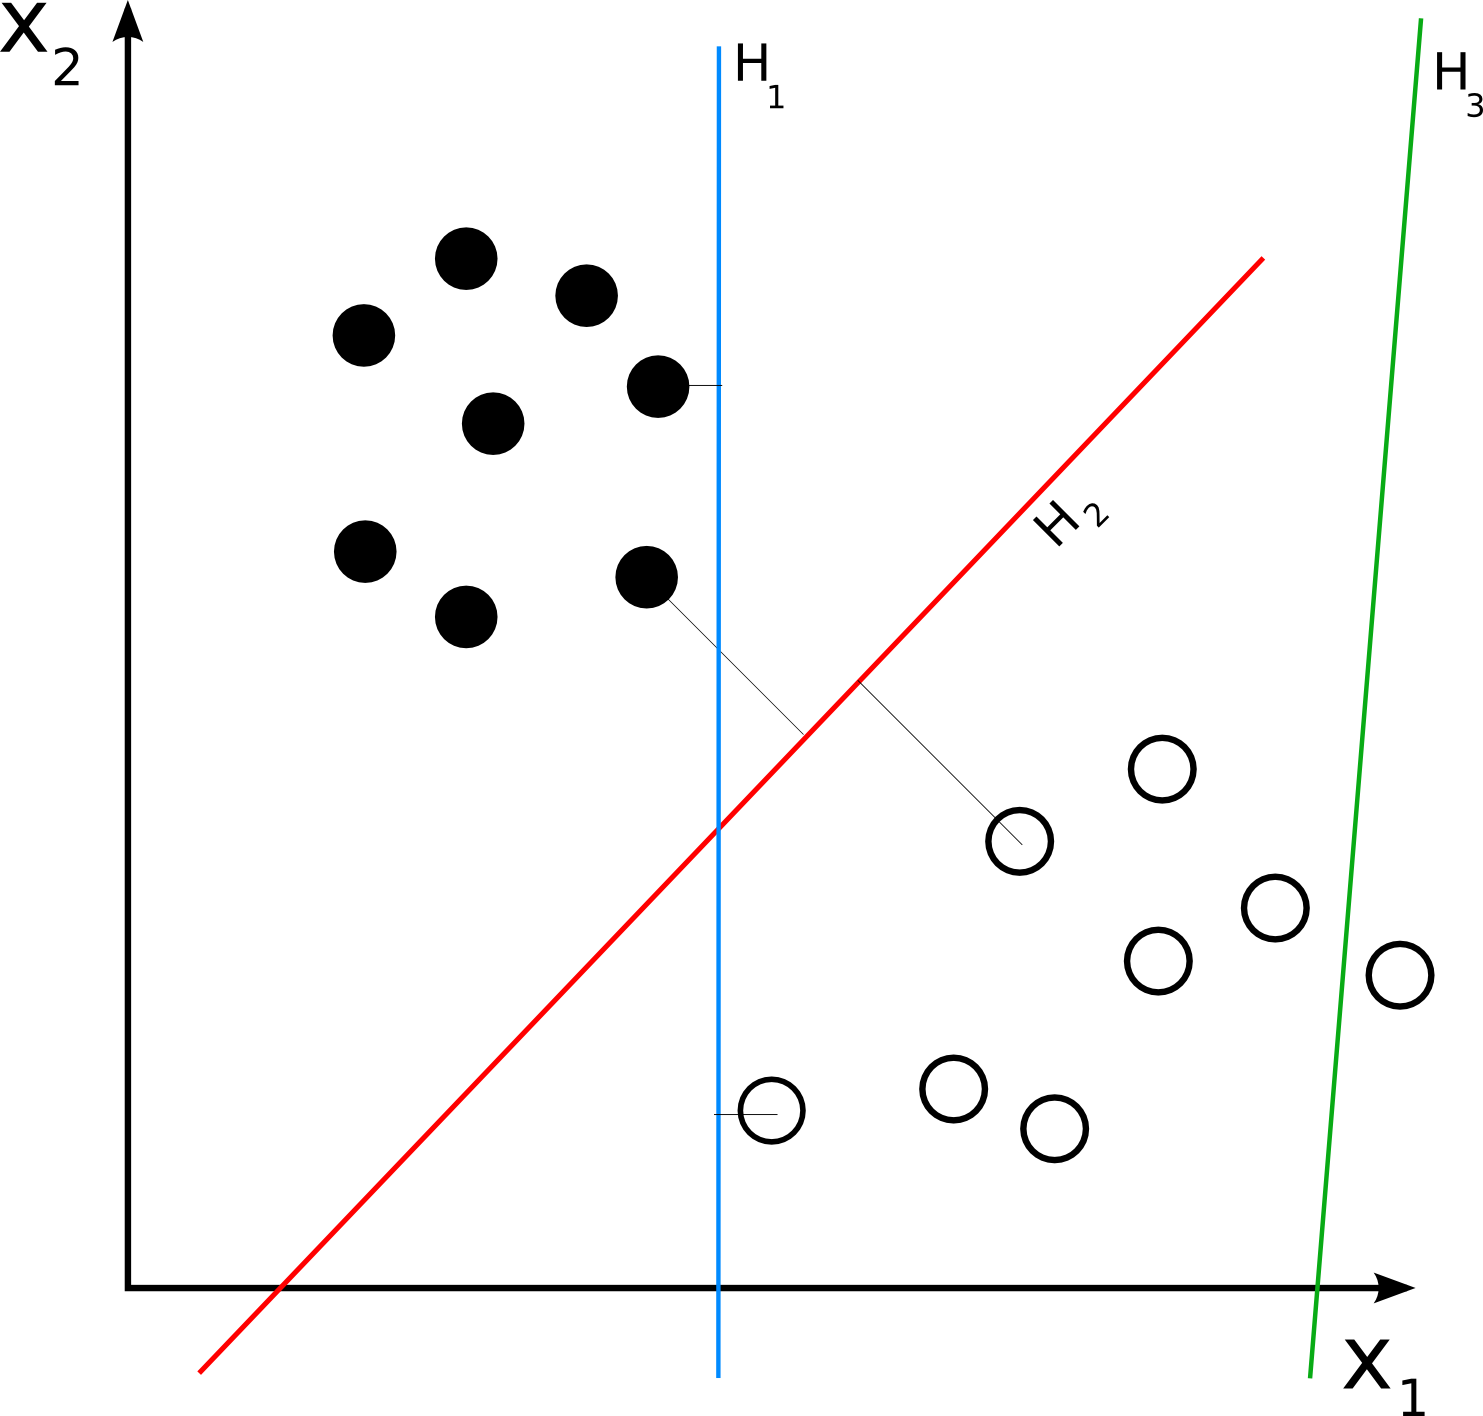
\includegraphics[scale=0.2]{Immagini/liblinear_esempio.png}
	\caption{Nella figura vediamo come il classificatore $H_1$ e $H_2$ classifichino
	correttamente i punti pieni e i punti vuoti. Potremo dire, inoltre, che $h_2$
	è un classificatore migliore perché la distanza media tra i vari elementi è costante}
	\label{fig:liblinearEx}
\end{figure}

\subsection{Liblinear}
Liblinear è una libreria opensource che implementa algoritmi di classificazione lineare. Il motivo
per cui è stato scelta come strumento per questa
tesi è principalmente dovuto la sua estesa documentazione, semplicità
d'uso, il suo già ampio utilizzo in ricerche simili e infine per la sua velocità nel calco dei risultati. In particolare l'ultimo punto si è rivelato fondamentale
per ottenere risultati in tempo ragionevole, in un confronto con un risoltuore \emph{SVM} (come \emph{LIBSVM})
i tempi di calcolo vengono ridotti di tre ordini di grandezza (da svariate ore a pochi secondi).

Liblinear supporta due popolari cassificatori binari \emph{LR, L2-regularized logistic regressione} e 
\emph{SVM L2-loss linear support vector machine}, dato un inseme di coppie
indicizzate $(x_i,y_i),i=1,\dot{},l,x_i\in R^n, y_i \in \{-1,+1\}$ entrambi i metodi risolvonolo stesso
problema di ottimizzazione senza vincoli ma con differenti \emph{loss functions} $\Xi(w;x_i,y_i)$:
\begin{equation}
	min_w \frac{1}{2}w^Tw+C\sum_i=1^l\Xi(w;x_i;y_i)
	\label{eqn:liblinear1}
\end{equation}

dove $C > 0$ è il parametro di penalità. Per \emph{SVM} le due \emph{loss functions} sono $max(1-y_iw^Tx_i,0)$ e
$max(1-y_iw^Tx_i,0)$. Per \emph{LR} invece abbiamo $\log(1+e^{-y_iw^Tx_i}$


\chapter{Raccolta dati}
La raccolta dati è stata svolta svolta partendo dal primo Gennaio 2015, i dati raccolti provengono da dodici canali twitch scelti in modo che rappresentassero un parte omogenea di informazioni.
In particolare sono stati scelti i due canali con maggiore audience dei quattro giochi con maggiore numero di spettatori della piattaforma Twitch.tv.
I canali sono tutit in lingua inglese e i dati sono stati raccolti modificando logging per IRC  in modo che potesse raccogliere dati attraverso il login e l'utilizzo dell API di twitch.
Oltre al messaggio di testo sono stati registrati anche l'autore (utente) del messaggio di testo, il timestamp e il canale nel quale il messaggio è stato inserito.

\section{Normalizzazione del corpus}
Dato il grande numero di dati e il fatto che chiunque può partecipare alla chat di Twitch si è reso necessario l'eliminazione degli eventuali messaggi di spam. Il primo step è stato quello di sostituire tutte gli URL presenti con il token \textbf{URL}. 
Il secondo step è stato quello di trasformare tutte le emoticons unicode presenti utilizzando il documento TODO LINK sostituendole con i rispettivi tag ASCII. Un'ulteriore step è stato preso in modo da eliminare caratteri unicode non necessari per esempio lettere straniere proveniennti da altri paesi non anglofoni (esempio \o, \oe, etc.).
Il principale metodo di tokenizzazione è stato fatto utilizzando \textbf{Twoketnizer} (TODO inserire link) un tokenizer sviluppato per tokenizzare testi provenienti da twitter. In particolare è stata utilizzata la sua implementazione in python con alcune modifiche in modo da trattare le emoticons presenti nel corpus di Twitch.

\section{Analisi Emoticons}
Sono state scelte per un'analisi più approfondita le seguenti emoticons:
\begin{table}[h]
\begin{center}
\begin{tabular}{|c|c|c|}
\hline
Nome Emoticon & Significato & Polarity \\
\hline
\hline
4Head & sarcasmo & positiva \\
\hline
anele & sarcasmo, in genere riferito alla cultura USA & neutra \\
\hline
babyrage & insofferenza & negativo \\
\hline
biblethump & disappunto & negativo \\
\hline
brokeback & sarcasmo & positiva \\
\hline
dansgame & critica & negativo \\
\hline
datsheffy & battute sulla polizia (singolo canale) & non considerato \\
\hline
elegiggle & sarcasmo & positiva \\
\hline
pogchamp & spam & non considerato \\
\hline
residentsleeper & noia & negative \\
\hline
smorc & tattiche relative ad un particolare gioco & neutra \\
\hline
swiftrage & rabbia & negativo \\
\hline
trihard & impegno &  neutro \\
\hline
wutface & spam & non considerato \\
\hline
failfish & disappunto & negative \\
\hline
frankerz & spam & non considerato \\
\hline
heyguys & annunci/saluti & positiva \\
\hline
kappa & sarcasmo & positiva \\
\hline
kappapride & sarcasmo & positiva \\
\hline
kreygasm & sarcasmo & positiva \\
\hline
mrdestructoid & battute / viewbotting & neutre \\
\hline
opieop & commenti sul cibo & neutra \\
\hline
osbury & offese & negativo \\
\hline
osrob & spam & non considerato \\
\hline
pjsalt & disappunto & negative \\
\hline
\end{tabular}
\end{center}
\caption{Analisi delle emoticons}
\label{tab:emoticons1}
\end{table}

Si può notare che è possibile divedere le emoticons in quattro classi separate, 
\begin{itemize}
\item Positiva: rappresenta frasi ironiche, sarcastiche e che esprimono un apprezzamento sul contenuto del canale.
\item Negativa: rappresenta un giudizio negativo sul contenuto del canale o su argomenti trattati in chat.
\item Neutra: sono emoticons che non hanno una polarity definita, in questa classe troviamo emoticons, per esempio opieop, utilizzate in frasi che parlano di cibo "I'm getting an hamburger now opieop" frasi che quindi sono scollegate dall'argomento dello streaming o della chat. In questa classe troviamo anche emoticons come mrdestructdroid che viene utilizzato principalmente per indicare il cosidetto "viewbotting" cioè l'utilizzo di software che crea connessioni fittizie allo streaming in modo da incrementare il numero di visualizzazioni in modo da far salire il ranking dello stream stesso. L'analisi di questo comportamento, anche se molto interessante, esula dagli argomenti trattati in questa tesi pertanto viene ignorato.
\item Non considerata: in questa classe troviamo le emoticons che non esprimono alcun giudizio, sono utilizzate spesso solo per creare "confusione" nella chat. TODO spiegare meglio
\end{itemize}

\begin{table}[h]
\begin{center}
\begin{tabular}{|c|c|c|}
\hline
Positive & Negative & Non considerate/Neutre \\
\hline
4Head & babyrage & datsheffy \\
\hline
anele &  biblethump &  pogchamp \\
\hline
brokeback &  dansgame & smorc \\
\hline
elegiggle & residentsleeper &  swiftrage \\
\hline
heyguys & failfish & trihard \\
\hline
kappa & pjsalt & wutface \\
\hline
kappapride & osbury & frankerz \\
\hline
kreygasm &  & keepo \\
\hline
 & & mrdestructoid \\
\hline
& & opieop \\
\hline
& & osrob \\
\hline
\end{tabular}
\end{center}
\caption{Lista di emoticons raggruppata per polarity}
\label{tab:emoticons2}
\end{table}

\chapter{Rnnlm}
\label{ch:rnnlm}
Seguento gli esempi pubblicati da Mikolov dove utilizza dati provenienti da IMDB e dimostra che un  modello generativo creato utilizzando recurrent neural network  può essere utilizzato per fare classificazione. Seguento lo stesso esempio sono creati modelli per ogni emoticons prendendo 15000 righe in modo casuale poi testati su un corpus di test composto da 25000 righe (diverse da quelle utilizzate come train).
Sono state prese 4 emoticons normalmente usate per esprimere un parere positivo e 6 per esmprimere un parere negativo e confrontate fra loro. Nelle tabelle sono rappresentate le percentuali di accurancy ottenuto sul file di test
\begin{table}[h]
\begin{center}
\begin{tabular}{|c|c|c|c|c|c|c|}
\hline
pos/neg & Babyrage & Biblethump & Dansgame & Failfish & notlikethis & wutface \\
\hline
\hline
4Head & 82.01 &  79.322 & 78 & 77 & 82.5 & 80.202 \\
\hline
Elegiggle & 84.372 & 83.696 & 80.794 & 77.454 & 84.7 & 84.288 \\
\hline
Kappa & 83.394 & 79.548 & 79.906 & 78.12 & 84.162 & 83.37 \\
\hline
Kreygasm & 84.944 & 81.964 & 80.388 & 82.228 & 84.608 & 81.114 \\
\hline
\end{tabular}
\end{center}
\caption{Confronto emoticons positive e negative}
\label{tab:rnnlmTest1}
\end{table}

Nello steso modo sono state confrontate le emoticon positive fra di loro
\begin{table}[h]
\begin{center}
\begin{tabular}{|c|c|c|c|c|}
\hline
pos/pos & 4Head & Elegiggle & Kappa & Kreygasm \\
\hline
\hline
4Head & 49.87 &  72.42 & 73.68 & 77.37 \\
\hline
Elegiggle & 72.126 & 50.37 & 78.58 & 81.98 \\
\hline
Kappa & 73.97 & 78.76 & 49.70 & 78.178 \\
\hline
Kreygasm & 77.41 & 82.8 & 79.178 & 49.62 \\
\hline
\end{tabular}
\end{center}
\caption{Confronto emoticons positive}
\label{tab:rnnlmTest2 }
\end{table}

Successivamente sono stati svolti i confronti tra tutte le emoticons positive e tutte quelle negative:
\afterpage{
\clearpage
\thispagestyle{empty}
\begin{landscape}
\centering
\begin{table}[h]
\begin{tabular}{|c|c|c|c|c|c|c|c|c|c|c|c|c|c|c|c|c|c|c|c|c|c|c|c|c|c|c|c|}
 & 4head & anele & babyrage & biblethump & brokeback & dansgame & datsheffy & elegiggle & failfish & frankerz & heyguys & kappapride & kappa & keepo & kreygasm & mrdestructoid & opieop & osbury & osrob & pjsalt & pogchamp & residentsleeper & smorc & swiftrage & trihard & wutface \\
4head &  49.638\% &  85.668\% &  82.05\% &  79.074\% &  76.462\% &  77.964\% &  90.016\% &  71.952\% &  77.076\% &  85.644\% &  85.906\% &  76.828\% &  74.556\% &  73.956\% &  77.214\% &  87.244\% &  79.09\% &  97.264\% &  94.782\% &  81.212\% &  73.688\% &  82.892\% &  &  &  & \\
anele &  &  49.962\% &  90.482\% &  88.012\% &  87.132\% &  88.236\% &  92.522\% &  88.9\% &  89.868\% &  87.402\% &  91.008\% &  85.584\% &  85.946\% &  85.866\% &  86.542\% &  90.804\% &  85.872\% &  97.146\% &  97.204\% &  89.542\% &  87.364\% &  91.866\% &  88.7\% &  90.362\% &  85.904\% &  88.028\%\\
babyrage &  &  &  50.094\% &  82.066\% &  84.308\% &  84.884\% &  93.334\% &  84.246\% &  84.112\% &  88.434\% &  90.384\% &  84.706\% &  83.196\% &  83.19\% &  84.616\% &  90.81\% &  85.408\% &  97.682\% &  96.252\% &  87.872\% &  83.644\% &  88.4\% &  87.298\% &  85.03\% &  89.026\% &  86.298\%\\
biblethump &  &  &  &  50.022\% &  83.162\% &  81.068\% &  91.722\% &  83.44\% &  82.318\% &  85.338\% &  88.02\% &  80.874\% &  79.278\% &  79.388\% &  81.566\% &  88.616\% &  82.164\% &  97.3\% &  95.134\% &  86.636\% &  80.894\% &  86.444\% &  86.02\% &  83.218\% &  86.318\% &  80.704\%\\
brokeback &  &  &  &  &  50.212\% &  80.112\% &  91.712\% &  79.862\% &  77.534\% &  87.13\% &  87.156\% &  80.892\% &  79.338\% &  78.786\% &  78.338\% &  89.308\% &  81.09\% &  96.934\% &  96.326\% &  84.73\% &  79.886\% &  84.766\% &  83.618\% &  86.012\% &  84.808\% &  81.72\%\\
dansgame &  &  &  &  &  &  50.188\% &  91.97\% &  81.268\% &  76.622\% &  87.676\% &  88.26\% &  81.818\% &  80.72\% &  80.136\% &  79.93\% &  89.924\% &  82.37\% &  97.694\% &  94.892\% &  86.99\% &  78.464\% &  85.474\% &  85.972\% &  82.058\% &  86.12\% &  76.998\%\\
datsheffy &  &  &  &  &  &  &  49.976\% &  90.514\% &  92.098\% &  92.186\% &  93.822\% &  91.234\% &  90.942\% &  90.406\% &  91.39\% &  93.002\% &  89.964\% &  98.184\% &  97.336\% &  93.192\% &  90.792\% &  93.486\% &  92.362\% &  92.488\% &  91.832\% &  92.448\% \\
elegiggle &  &  &  &  &  &  &  &  49.942\% &  78.47\% &  89.74\% &  89.276\% &  82.63\% &  79.42\% &  79.698\% &  82.324\% &  89.884\% &  82.878\% &  97.276\% &  94.734\% &  85.352\% &  79.718\% &  85.376\% &  86.694\% &  85.15\% &  87.324\% &  84.292\%\\
failfish &  &  &  &  &  &  &  &  &  49.9\% &  89.344\% &  89.636\% &  83.634\% &  78.926\% &  78.448\% &  81.096\% &  90.666\% &  83.182\% &  97.756\% &  95.738\% &  86.544\% &  80.558\% &  84.358\% &  84.07\% &  85.022\% &  87.616\% &  81.916\%\\
frankerz &  &  &  &  &  &  &  &  &  &  49.89\% &  89.774\% &  83.898\% &  85.302\% &  82.472\% &  87.604\% &  89.27\% &  84.768\% &  97.106\% &  97.068\% &  86.454\% &  87.176\% &  90.716\% &  88.694\% &  90.114\% &  86.466\% &  88.002\%\\
heyguys &  &  &  &  &  &  &  &  &  &  &  49.85\% &  86.042\% &  87.862\% &  86.734\% &  85.712\% &  92.036\% &  87.23\% &  97.426\% &  97.166\% &  90.164\% &  86.326\% &  91.948\% &  91.41\% &  91.314\% &  89.478\% &  88.52\%\\
kappapride &  &  &  &  &  &  &  &  &  &  &  &  50.264\% &  &  75.91\% &  79.28\% &  88.798\% &  80.438\% &  97.046\% &  95.992\% &  84.532\% &  79.836\% &  87.022\% &  85.314\% &  85.18\% &  84.066\% &  82.592\%\\
kappa &  &  &  &  &  &  &  &  &  &  &  &  76.268\% &  49.902\% &  71.292\% &  78.71\% &  87.22\% &  78.298\% &  97.572\% &  95.2\% &  84.958\% &  77.112\% &  84.758\% &  82.486\% &  84.074\% &  84.852\% &  82.796\%\\
keepo &  &  &  &  &  &  &  &  &  &  &  &  &  &  50.368\% &  78.54\% &  87.052\% &  77.286\% &  97.492\% &  96.352\% &  83.93\% &  78.416\% &  85.408\% &  82.802\% &  84.166\% &  83.648\% &  82.418\%\\
kreygasm &  &  &  &  &  &  &  &  &  &  &  &  &  &  &  50.004\% &  87.99\% &  81.662\% &  97.566\% &  95.404\% &  85.918\% &  71.374\% &  85.754\% &  84.664\% &  83.842\% &  83.504\% &  81.59\%\\
mrdestructoid &  &  &  &  &  &  &  &  &  &  &  &  &  &  &  &  49.868\% &  89.116\% &  97.898\% &  97.268\% &  91.098\% &  89.688\% &  91.228\% &  90.71\% &  90.454\% &  89.44\% &  90.524\%\\
opieop &  &  &  &  &  &  &  &  &  &  &  &  &  &  &  &  &  49.73\% &  97.68\% &  95.226\% &  86.306\% &  80.384\% &  87.346\% &  85.158\% &  87.116\% &  83.586\% &  84.342\%\\
osbury &  &  &  &  &  &  &  &  &  &  &  &  &  &  &  &  &  &  49.96\% &  98.856\% &  97.538\% &  97.518\% &  98.064\% &  97.954\% &  97.672\% &  97.298\% &  97.424\%\\
osrob &  &  &  &  &  &  &  &  &  &  &  &  &  &  &  &  &  &  &  49.988\% &  96.822\% &  96.118\% &  97.134\% &  95.87\% &  96.11\% &  96.548\% &  96.582\%\\
pjsalt &  &  &  &  &  &  &  &  &  &  &  &  &  &  &  &  &  &  &  &  50.068\% &  85.194\% &  89.502\% &  88.208\% &  89.998\% &  87.598\% &  87.048\%\\
pogchamp &  &  &  &  &  &  &  &  &  &  &  &  &  &  &  &  &  &  &  &  &  50.348\% &  85.058\% &  84.184\% &  81.532\% &  85.13\% &  80.16\%\\
residentsleeper &  &  &  &  &  &  &  &  &  &  &  &  &  &  &  &  &  &  &  &  &  &  50.17\% &  88.79\% &  88.07\% &  89.22\% &  87.948\%\\
smorc &  &  &  &  &  &  &  &  &  &  &  &  &  &  &  &  &  &  &  &  &  &  &  49.91\% &  86.068\% &  87.62\% &  86.966\%\\
swiftrage &  &  &  &  &  &  &  &  &  &  &  &  &  &  &  &  &  &  &  &  &  &  &  &  49.776\% &  89.082\% &  85.906\%\\
trihard &  &  &  &  &  &  &  &  &  &  &  &  &  &  &  &  &  &  &  &  &  &  &  &  &  50.014\% &  84.77\%\\
wutface &  &  &  &  &  &  &  &  &  &  &  &  &  &  &  &  &  &  &  &  &  &  &  &  &  &  49.804\%\\
\end{tabular}
\caption{Confronto emoticon globale}
\label{tab:rnnlmTest3 }
\end{table}
\end{landscape}
\clearpage
}

In questo modo è facile notare che non solo rnnlm riesce a distinguere con alta probabilita  tra frasi provenienti da emoticons positive e quelle da emoticons negative. Ma riesce anche a distinguere con elevata precisione anche le differenze tra due diverse emoticons positive.
\chapter{Liblinear}
\label{ch:liblinear}
Per generare i risultati attraverso liblinear è stato utilizzato word2vec con la patch di Mikolov per i sentence vectors. Similmente da come è stato effettuato con rnnlm sono stati creati file di training e test partendo dalle frasi derivate da due differenti emoticons, una positiva e un'altra negative contenenti 12500 righe ciascuno. Successivamente sono stati creati i file di test di lunghezza 25000 righe. Nonostante nei test sia stato utilizzato un sottoinsieme dei dati i vettori sono stati creati utilizzando l'intero corpus.
Sono state effettuate alcune prove cambiando la lunghezza dei vettori (da 100 a 300 elementi) e anche utilizzando sia l'algoritmo c-bow che continous skipgram. Non sono state osservate particolari differenze nei risultati, per questo motivo si è scelto di utilizzare vettori da 100 elementi e l'algoritmo skipgram.
Come effettuato nel Capitolo 2 sono state effettuati i confronti tra coppie di emoticons positive e negative:

\begin{table}[h]
\begin{center}
\begin{tabular}{|c|c|c|c|c|c|c|}
\hline
pos/neg & Babyrage & Biblethump & Dansgame & Failfish & notlikethis & wutface \\
\hline
\hline
4Head & 67.01 &  69.322 & 78 & 67 & 65.5 & 70.202 \\
\hline
Elegiggle & 69.37 & 71.696 & 70.74 & 67.54 & 69.7 & 68.28 \\
\hline
Kappa & 70.94 & 69.548 & 69.906 & 68.12 & 68.162 & 71.37 \\
\hline
Kreygasm & 69.44 & 71.96 & 70.33 & 72.43 & 67.76 & 71.32 \\
\hline
\end{tabular}
\end{center}
\caption{Confronto emoticons positive e negative}
\label{tab:liblinearTest1}
\end{table}

Sono stati effettuati anche alcuni test utilizzando tutti i vari algoritmi disponibili da liblinear; questo test è stato svolto utilizzando tutti i parametri di default e testato con tutti gli algoritmi la seconda colonna rappresenta i risulati ottenuti con -c 2
\begin{table}[h]
\begin{center}
\begin{tabular}{|l|c|r|}
\hline
Algoritmo & c  default & -c 2 \\
\hline
\hline
0 & 66.9 & 66.88\\
\hline
1 & 66.93 & 66.95\\
\hline
2 & 66.93 & 67.14\\
\hline
3 & 67.16 & 67.24\\
\hline
4 & 67.15 & 66.93\\
\hline
5 & 66.94 & 66.90\\
\hline
6 & 66.9 & 66.84\\
\hline
7 & 66.90 & 66.89\\
\hline
11 & 66.93 & 66.93\\
\hline
12 & 66.47 & 66.63\\
\hline
13 & 65.188 & 67.02\\
\hline
\end{tabular}
\end{center}
\caption{test liblinear}
\label{tab:liblineraTest1}
\end{table}

Il parametro C è stato ricercato utililzzando la funzionalità di liblinear -C: ./train -s 0 -C train.txt . Il risultato ottenuto è stato un c pari a 2. Un ulteriore test utilizzando l'algoritmo 2 e modificando i c da 1 a 4 non ha portato alcuna differenza nei valori di precisione.

TODO inserire i grafici creati con t-sne per la vicinanza delle emoticons

\chapter{Risultati}
I test conclusivi per la classificazione di polarità sono stati effettiati eseguendo sia \textbf{rnnlm} e poi successivamente \textbf{word2vec e liblinear} sullo stesso set di dati. Da come è stato possibile leggere nei capitoli precedenti sono stati eseguiti due test: il primo utilizzando i dati della tabella  \ref{tab:rnnlmTest1}, mentre il secondo è stato svolto utililzando tutte le emoticons positive e negative descritte nella tabella \ref{tab:emoticons1}. 
I test sono stati sempre svolti con un corpus di training di 12500 righe per file (file positivo e negativo) scelte casualmente tra tutto il corpus e un test di 25000 per file. I sentence vectors sono stati generati utililzando l'intero corpus di emoticons positive, negative e neutre non limitato al numero di righe prese in considerazione per i file di training e test.
I risultati ottenuti sono i seguenti:
\begin{table}[h]
\begin{center}
\begin{tabular}{|c|c|c|c|}
\hline
& rnnlm & c liblinear & totale \\
\hline
no ripetizioni 1 & 72.53 & 66.50 & 75.85  \\
\hline
no ripetizioni 2 & 73.34 & 67.50 & 74.85  \\
\hline
no ripetizioni 3 & 72.13 & 66.78 & 75.01  \\
\hline
standard 1 & 74.52 & 67.01 & 78.89 \\
\hline
standard 2 & 75.33 & 69.23 & 81.01 \\
\hline
standard 3 & 74.92 & 68.33 & 79.90 \\
\hline
\end{tabular}
\end{center}
\caption{test liblinear}
\label{tab:test1}
\end{table}

In questo caso sono stati ripetuti 3 volte i test, utilizzando un set di dati di training e test diverso per ogni test. In particolare è stato effettuato un set test rimuovendo le ripetizioni nelle stasse frase. Questo meccanismo, oltre ad alterare il corpus originale, porta a valori di precisione leggermente inferiori e quindi è stato scartato dai successivi test.
\begin{es}
Eliminazione di ripetizione: In una frase contenente le seguenti parole:  ``Good Game Kappa Good Game Kappa Good Game Kappa`` è stata ridotta eliminando le parole ripetute ad una frase del tipo ``Good Game Kappa``.
\end{es}

\section{Analisi di più emoticons}
E' stato suddiviso il corpus in due parti: una parte contenente tutte le frasi positive: cioè quelle contenenti una delle emoticons citate nella tabella \ref{tab:rnnlmTest1} e quello negativo costriuto in egual modo ma utilizzando le frasi marcate con emoticons negative. Questi due set di dati sono statati randomizzati in modo che le frasi proveninenti dalle differenti emoticons venissero considerate con uguale probabilità. Sono state prese 25000 righe da entrambi i file ed effetuando lo stesso procedimento utilizzato nei capitoli \ref{ch:rnnlm} e \ref{ch:liblinear} è stato fatto il training sia con rnnlm che con liblinear, dopo aver processato i vettori (costruiti con l'intero corpus positivo, negativo e neutro).
I test sono stati effettuati utilizzando altre 25000 righe provenienti da entrambi i file positivi e negativi (tutte frasi differenti da quelle utilizzate per il training). Il risultato ottenuto è riportato nella tabella \ref{tab:test2}.
\begin{table}[h]
\begin{center}
\begin{tabular}{|c|c|c|c|}
\hline
& rnnlm & c liblinear & totale \\
\hline
\hline
Test 1 & 54.20 & 52.32 & 53.30 \\
\hline
Test 2 & 53.32 &  51.50 &  53.85  \\
\hline
Test 3 & 53.20 & 52.01 &  51.89 \\
\hline
\end{tabular}
\end{center}
\caption{test liblinear}
\label{tab:test2}
\end{table}

I risultati cosi bassi sono dovuti al fatto che, anche se concettualmente le emoticons positive esprimono una polarità positiva in realtà la costruzione delle frasi associate sono molto diverse. 
In altre parole il sistema si ``confonde`` tra le varie emoticons positive e quelle negative. Come indicato nelle tabelle del capitolo \ref{ch:rnnlm} è facile vedere che l'algoritmo riece a differenziare molto bene anche tra emoticons che esprimono lo stesso giudizio (positivo o negativo). Utilizzando frasi provenienti da tutte queste emoticon il training considera della stessa ``distanza`` sia le eventuali emoticons positive che quelle negative e riesce a distinguere le frasi in maniera molto meno precisa.

\section{Miglioramento risultati analisi con più emoticons}
Sono state fatte numerose prove per migliorare la precisione del risultato, la soluzione utilizzata, cioè quella che ha raggiunto un livello di accurancy più alta è stata la seguente:
Sono state suddivise le frasi per ogni emoticons considerata: quindi il corpus è stato suddiviso in 7 file positivi e 8 negativi. Prendendo 12500 righe casuali da ognuno di questi file è stato generato un modello per ogni singolo file utilizzando rnnlm e liblinear.(I vettori utilizzati per liblinear sono stati sempre costruiti nel solito modo tenendo conto dell'intero corpus quindi anche delle frasi neutre). In questo modo sono stati ottenuti 8 modelli per le emoticons negative e 7 per le emoticons negative.
Per il test sono state prese 25000 righe di emoticons positive e altrettante negative in maniera casuale tra tutte quelle delle emoticons positive e negative ed in questo modo è stato creato il file di test. Questo file di test è stato confrontato con ogni combinazione di modelli positivo-negativo generati e sono stati salvati tutti i risultati parziali.
\begin{es}
Consideriamo le emoticon trattate:
\begin{itemize}
\item Positive: kappa, 4head, elegiggle, kappapride, kreygasm, heyguys, anele
\item Negative: residentsleeper, pjsalt, wutface, notlikethis, failfish, biblethump, dansgame, babyrage
\end{itemize}
Il file di test viene processato usando come modello di training ogni confronto tra emoticons, quindi prima ottengo il risultato processando il file con il modello kappa-residentsleeper, poi kappa-pjsalt, kappa-wutface etc. In questo modo ottengo 56 risultati differenti che rappresentano tutti le possibili combinazioni di confronti tra emoticons positive con quelle negative.
\end{es}

In questo modo sono state ottenui 56 risultati parziali per ogni riga del file di test, questi risultati parziali sono stati confrontati facendo la sommatoria di quelli che hanno dato esito positivo con quelli che hanno dato esito negativo, se è stata ottenuta la maggioranza di risultati positivi allora alla frase è stato attribuito un punteggio positivo, se invece la maggioranza risultate negativo è stato attribuito un valore negativo. In caso di pareggio il valore assegnato è neutro.
Utilizzando questa procedura i valori ottenuti sono paragonabili a quelli del  test singolo fatto in precedenza:
\begin{table}[h]
\begin{center}
\begin{tabular}{|c|c|c|c|}
\hline
& rnnlm & liblinear & totale \\
\hline
\hline
Test 1 & 70.20 & 61.32 & 72.30 \\
\hline
Test 2 & 72.53 & 60.40 & 73.85  \\
\hline
Test 3 & 72.52 & 62.01 & 73.89 \\
\hline
\end{tabular}
\end{center}
\caption{test liblinear}
\label{tab:test3}
\end{table}

\section{Baseline}
Come baseline è stato effettuato, sugli stessi dati utilizzati nel test precendente, un BOW utilizzando Weka e processando i risultati utilizzando liblinear con gli stessi parametri utilizzati per per word2vec. I risultati sono indicati nella tabella \ref{tab:baseTest1}
\begin{table}[h]
\begin{center}
\begin{tabular}{|c|c|}
\hline
& risultato  \\
\hline
\hline
Test 1 & 62.22 \\
\hline
Test 2 & 63.56 \\
\hline
Test 3 & 63.41 \\
\hline
\end{tabular}
\end{center}
\caption{test bow}
\label{tab:baseTest1}
\end{table}

Si può vedere che utilizzando il bow i risultati sono circa di 10 punti percentuali inferiori a quelli ottenuti utilizzando rnnlm, word2vec e liblinear
\chapter{Analisi dell'andamento giornaliero}
Sono state analizzate le chat e i video prodotti da alcuni streamer nell'intero arco della giornata. I dati sono stati processati dapprima utilizzando il tokenizzatore e poi rimuovendo le emoticons. L'intera giornata è stata suddivisa in intervalli di 5 minuti, per ogni intervallo sono state calcolate le somme di tutte le frasi positive, negative e neutre. Questo a permesso di ottenere un grafico dell'andamento della giornata.
E' stato calcolato anche anche uno stesso andamento utilizzando lo stesso corpus, questa volta senza aver eliminato le emoticons utilizzando un semplice algoritmo che considera solo il numero di emoticons presenit in ogni frase. ES: in una frase ci sono 3 emoticons positive e 1 negativa allora assumo che la frase sia positiva.
Come test iniziale sono stati analizate tre giornate di tre differenti persone:
\newline
\newline
Per ora i dati sono centenuti nei tre excel: il primo foglio rappresenta i dati generati utilizzando l'algoritmo rnnlm, word2vec, liblinear, il secondo foglio rappresenta i dati generati solo dal calcolo delle emoticons e nel terzo fogli ci sono i 3 grafici: l'andamento utilizzando l'algoritmo, l'andamento utilizzando solo le emoticons e infine il confronto tra l'andamento generato dall'algoritmo e dalle sole emoticons.

Vediamo il file \emph{1\_6\_amazhs.xlsx}, durante questa giornata tutti i commenti in chat sono riferiti ad eventi nello stream (vittorie, sconfitte) e l'utilizzo estremamente elevato di emoticons ha portato ad una eguagliana piuttosto elevata dai dati ottenuti solamente dall'analisi delle emoticons. I vari picchi sono stati verificati manualmente e rappresentavano correttamente eventi positivi o negativi

Nei due file successivi \emph{1\_4\_destiny.xlsx} e \emph{1\_7\_massansc.xlsx} vediamo come l'analisi delle sole emoticons non è più sufficiente. La divergenza è dovuta al fatto che l'utilizzo in chat di emoticons è relativamente basso rispetto al numero di messaggi, la polarity generata con rnnlm/word2vec tiene conto anche dei messaggi senza emoticons. Con un controllo manuale nei vari picchi è risultato che la polarity rilevata da rnnlm/word2vec è effettivamente quella corretta, in più viene rilevata correttamente sia la polarità degli eventi dello stream che dei meta-eventi (disconnessioni, problemi tecnici etc. vedi capitolo \ref{ch:sviluppi}

\chapter{Sviluppi}
\label{ch:sviluppi}
\begin{itemize}
\item Nell'analisi delle emoticons multiple invece di fare una semplice ``binary decision`` cioè contare il numero di volte che è stato assegnato un valore positivo e negative e assegnare la polarità a seconda del risultato della differenza tra i due valori si potrebbe utilizzare liblinear per creare un modello intermedio per i 56 risultati usato poi per classificare i risultati generati dal file di test.
\item Nei grafici finali aggiungere anche il grafico dell'andamento della polarity calcolato con la baseline (bow + liblinear)
\item Analisi della meta-polarità: facendo verifice manuali su i dati finali ottenuti è risultato che si potrebbe fare un'analisi in due livelli: il primo livello rappresenta la polarità del contenuto dello stream, per esempio se nello stream avviene un evento positivo (es. una vittoria) o negativo (es. una sconfitta) la chat reagisce di conseguenza aumentado il numero di commenti positivi o negativi.
Si è visto che è presente anche un secondo livello, un meta-livello, dove le frasi scritte in chat (quindi anche la polarita) è riferita ad eventi che esulano dai contenuti dello stream, ma l'oggetto della discussione riguarda lo stream stesso (es: ``Stream quality sucks!'' [negativa] oppure ``The song yoùre playing is amazing!'' [positiva], ``you are cheating!'' [negativa] etc.).
\end{itemize}
\end{document}
